\chapter{Integración del LDAP del clúster con el WordPress}
%%%%%%%%%%%%%%%%%%%%%%%%%%%%%%%%%%%%%%%%%%%%%%%%%%%%%%%%%%%%%%%%%%%%%
En este capítulo se cubre la integración de los usuarios del protocolo ligero de acceso a directorios (LDAP) propios del clúster, al WordPress del clúster, para facilitar el uso del sistema de soporte sin necesidad de mantener usuarios duplicados en sistemas separados.
%%%%%%%%%%%%%%%%%%%%%%%%%%%%%%%%%%%%%%%%%%%%%%%%%%%%%%%%%%%%%%%%%%%%%
En general, un LDAP es un estándar de protocolo de aplicación para el acceso y mantenimiento de servicios de información de directorios distribuido, el cual funciona sobre IP, por lo cual puede ser  considerado una base de datos, pero especialmente orientada al manejo de datos de usuarios en un sistema LAN \cite{openldap}\cite{whatldap}.
%%%%%%%%%%%%%%%%%%%%%%%%%%%%%%%%%%%%%%%%%%%%%%%%%%%%%%%%%%%%%%%%%%%%%
Es posible integrar este sistema a la lista de usuarios del WordPress mediante la instalación de un plugin al sitio. Los pasos detallados se muestran más adelante. Se asume que se tiene acceso a través de SSH o de forma directa  al clúster, así como acceso a root a través de contraseña o mediante sudo, para poder trabajar. Para iniciar sesión por SSH se debe hacer lo siguiente:
%%%%%%%%%%%%%%%%%%%%%%%%%%%%%%%%%%%%%%%%%%%%%%%%%%%%%%%%%%%%%%%%%%%%%
\begin{lstlisting} 
user@localhost ~ $ ssh -p 22 usuario@cluster.cenat.ac.cr
[date - user@meta:~ ] $ su -
[date - root@meta:~ ] $ 
\end{lstlisting}
%%%%%%%%%%%%%%%%%%%%%%%%%%%%%%%%%%%%%%%%%%%%%%%%%%%%%%%%%%%%%%%%%%%%%

Antes que nada, es necesario preparar el sitio web para trabajar con LDAP de forma nativa. para ello se debe instalar el paquete php-ldap.
%%%%%%%%%%%%%%%%%%%%%%%%%%%%%%%%%%%%%%%%%%%%%%%%%%%%%%%%%%%%%%%%%%%%%
\begin{lstlisting} 
yum install php-ldap
service httpd restart
\end{lstlisting}
%%%%%%%%%%%%%%%%%%%%%%%%%%%%%%%%%%%%%%%%%%%%%%%%%%%%%%%%%%%%%%%%%%%%%
Con esto listo,  procedemos a descargar e instalar el plugin wpdirauth \cite{pluginldap}. Tome en cuenta que la versión descrita acá puede variar en el futuro, por lo que  cualquier cambio o actualización deberá documentarse y probarse para garantizar que sigue siendo compatible con la configuración del clúster.
%%%%%%%%%%%%%%%%%%%%%%%%%%%%%%%%%%%%%%%%%%%%%%%%%%%%%%%%%%%%%%%%%%%%%
\begin{lstlisting} 
wget https://downloads.wordpress.org/plugin/wpdirauth.1.7.15.zip
unzip wpdirauth.1.7.15.zip
mv wpdirauth /var/www/html/wordpress/wp-content/plugins
\end{lstlisting}
%%%%%%%%%%%%%%%%%%%%%%%%%%%%%%%%%%%%%%%%%%%%%%%%%%%%%%%%%%%%%%%%%%%%%
Una vez hecho lo anterior, ingresamos a la página del WordPress del clúster \url{http://cluster.cenat.ac.cr/wordpress/wp-admin/}. Debería aparecernos un prompt como el de la figura \ref{fig:ldap:01}. En esta instancia se requiere tener una cuenta por aparte para acceder  al wp-admin del sitio del clúster, por lo que si no la tiene aún, es  recomendable solicitarla al administrador a cargo.
%%%%%%%%%%%%%%%%%%%%%%%%%%%%%%%%%%%%%%%%%%%%%%%%%%%%%%%%%%%%%%%%%%%%%
\begin{figure}[H]
\centering
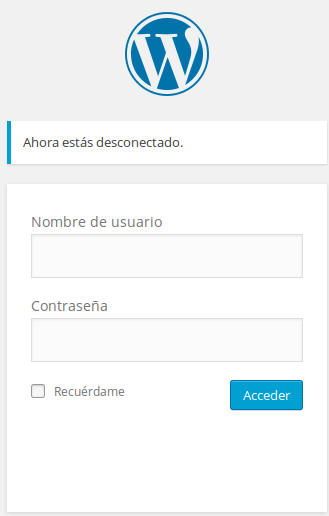
\includegraphics[width=0.3\textwidth]{wp_login.png}
\caption{Inicio de sesión del wp-admin.}
\label{fig:ldap:01}
\end{figure}
%%%%%%%%%%%%%%%%%%%%%%%%%%%%%%%%%%%%%%%%%%%%%%%%%%%%%%%%%%%%%%%%%%%%%
Una vez ingresado, nos dirigimos al menú de plugins al lado izquierdo haciendo clic. Dentro nos aparecerá una lista de plugins previamente instalados y ahora aparecerá el plugin que acabamos de agregar, wpdirauth. Para habilitarlo simplemente hacemos clic en activar, como se muestra en la figura \ref{fig:ldap:02}.
%%%%%%%%%%%%%%%%%%%%%%%%%%%%%%%%%%%%%%%%%%%%%%%%%%%%%%%%%%%%%%%%%%%%%
\begin{figure}[H]
\centering
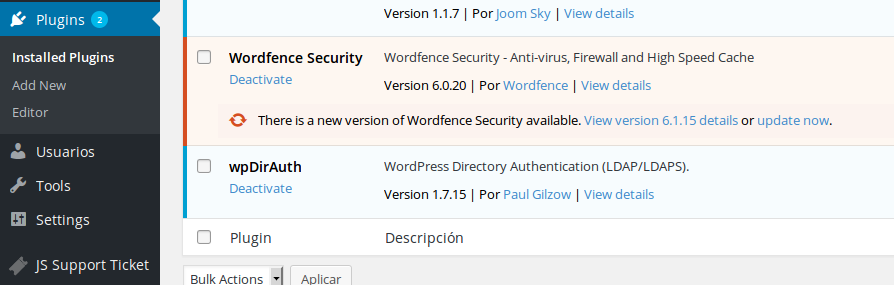
\includegraphics[width=0.5\textwidth]{ldap_plugin_activate.png}
\caption{Activación de plugin wpdirauth para sincronizar el LDAP.}
\label{fig:ldap:02}
\end{figure}
%%%%%%%%%%%%%%%%%%%%%%%%%%%%%%%%%%%%%%%%%%%%%%%%%%%%%%%%%%%%%%%%%%%%%
Actualizamos la página (F5) y nos dirigimos al menú Settings/Ajustes y luego hacemos clic en Directory Auth, como se muestra en la figura \ref{fig:ldap:03}. 
%%%%%%%%%%%%%%%%%%%%%%%%%%%%%%%%%%%%%%%%%%%%%%%%%%%%%%%%%%%%%%%%%%%%%
\begin{figure}[H]
\centering
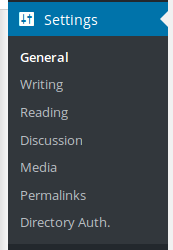
\includegraphics[width=0.35\textwidth]{ldap_plugin_settings00.png}
\caption{Ingreso a la configuración del plugin wpdirauth.}
\label{fig:ldap:03}
\end{figure}
%%%%%%%%%%%%%%%%%%%%%%%%%%%%%%%%%%%%%%%%%%%%%%%%%%%%%%%%%%%%%%%%%%%%%
Una vez dentro, procedemos a configurar el plugin para que funcione sin problemas con el LDAP.
%%%%%%%%%%%%%%%%%%%%%%%%%%%%%%%%%%%%%%%%%%%%%%%%%%%%%%%%%%%%%%%%%%%%%
\begin{itemize}
\item Enable Directory Authentication?: Yes
\item Require SSL Login?: No
\item Automatically Register Authenticated Users?: Yes
\item Enable SSL COnectivity?: No SSL Connectivity
\item Directory Servers (Domain Controllers): 10.0.0.1,0.0.0.0
\item Account Filter: uid
\item Base DN: dc=cnca,dc=cenat
\end{itemize}
%%%%%%%%%%%%%%%%%%%%%%%%%%%%%%%%%%%%%%%%%%%%%%%%%%%%%%%%%%%%%%%%%%%%%
Las opciones de Branding Settings son misceláneas pero deseables. En las figuras \ref{fig:ldap:04} y \ref{fig:ldap:05} se resume lo que se debe hacer. Una vez hechos los cambios, no olvide hacer clic en Update Options al inicio o al final de la página para cargar  los ajustes \cite{wpldap}.
%%%%%%%%%%%%%%%%%%%%%%%%%%%%%%%%%%%%%%%%%%%%%%%%%%%%%%%%%%%%%%%%%%%%%
\begin{figure}[H]
\centering
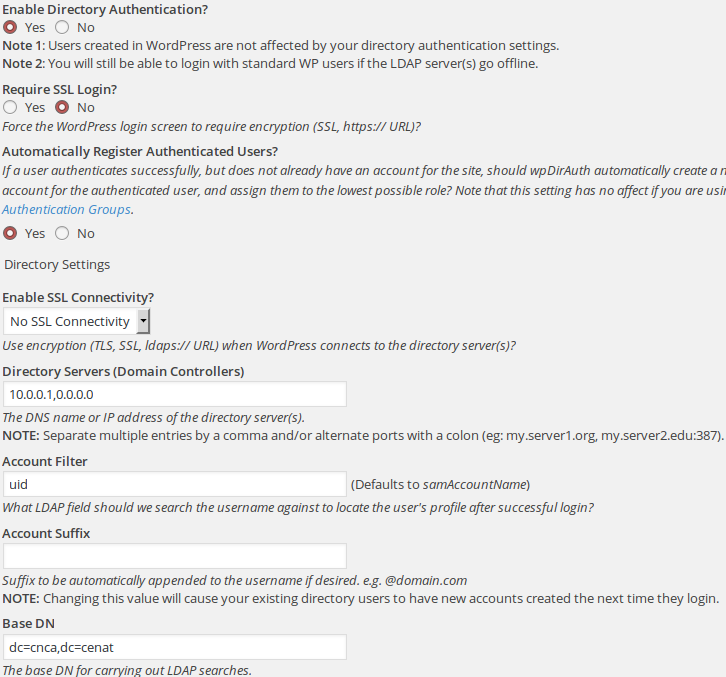
\includegraphics[width=0.6\textwidth]{ldap_plugin_settings01.png}
\caption{Ajustes básicos para tener un sistema de autenticación funcional con LDAP.}
\label{fig:ldap:04}
\end{figure}
%%%%%%%%%%%%%%%%%%%%%%%%%%%%%%%%%%%%%%%%%%%%%%%%%%%%%%%%%%%%%%%%%%%%%
\begin{figure}[H]
\centering
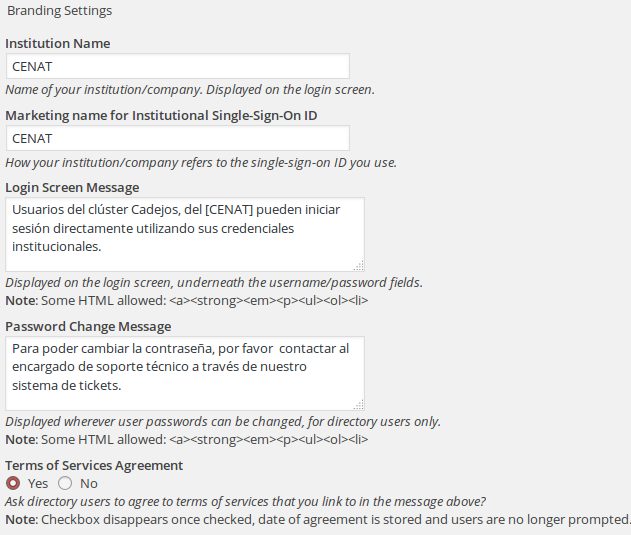
\includegraphics[width=0.6\textwidth]{ldap_plugin_settings02.png}
\caption{Branding Settings para formalizar el proceso de inicio de sesión.}
\label{fig:ldap:05}
\end{figure}
%%%%%%%%%%%%%%%%%%%%%%%%%%%%%%%%%%%%%%%%%%%%%%%%%%%%%%%%%%%%%%%%%%%%%
Si se han seguido los pasos descritos, el LDAP debería haberse  integrado satisfactoriamente al wordpress. Cierre sesión e intente ingresar con una cuenta verificada del LDAP, como se muestra en la  figura \ref{fig:ldap:06}.
%%%%%%%%%%%%%%%%%%%%%%%%%%%%%%%%%%%%%%%%%%%%%%%%%%%%%%%%%%%%%%%%%%%%%
\begin{figure}[H]
\centering
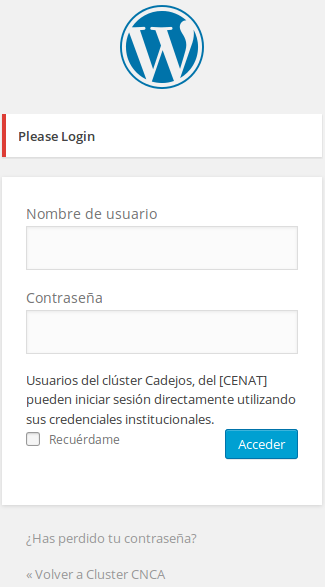
\includegraphics[width=0.35\textwidth]{ldap_plugin_settings03.png}
\caption{Pantalla de inicio de sesión con el plugin wpdirauth activado y funcionando.}
\label{fig:ldap:06}
\end{figure}
%%%%%%%%%%%%%%%%%%%%%%%%%%%%%%%%%%%%%%%%%%%%%%%%%%%%%%%%%%%%%%%%%%%%%
\clearpage